\documentclass[Skript.tex]{subfiles} 
\begin{document}


\section{Aufbau}

\subsection{Spielbeschreibung}

\gname ist ein Platformer bei dem über eine eingelesene Musikdatei die Karte generiert.
Der Spieler muss Genre typisch Hindernissen ausweichen.

Als geschichtlicher Hintergrund wir hier die Flucht vor der Arbeit (Hausaufgabe etc.\ ) genutzt. 
Der Spieler versucht anhand seiner Musik und dem Spiel, Zeit tot zu schlagen.

Der Designschwerpunkt des Spiels \gname liegt in der Idee das der Spieler eine gewünschte Musikdatei einlesen kann und die daraus generierte Karte im Anschluss spielt. 
Während der Spieler sich durch das Level bewegt soll passend dazu seine vorher eingelesene Musik abgespielt werden.

Das Grundgameplay besteht aus dem Ziel Hindernissen solange auszuweichen bis das Lied vorbei ist. 

\subsection{Visuelle Präsentation}
\begin{wrapfigure}[9]{r}{4cm}
\vspace{-1.2cm}
  \begin{center}
    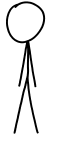
\includegraphics[scale=.9]{Grafik/char.png}
	\caption{Standard Charakter}
	\label{charakter}
  \end{center}
\end{wrapfigure}

Der Stil des Spiels \gname soll sich an die Comics von \textit{Randall Munroe} anlehnen.
Hier dienen die Charaktere von \href{http://xkcd.com}{xkcd.com}.




Die Lizenz \href{http://creativecommons.org/licenses/by-nc/2.5/}{creativecommons.org} erlaubt uns Material mitzubenutzen und  zu verändern.
Voraussetzung dafür ist darauf zu verweisen (Webseite, Lizenz) und kein Kommerziellen nutzen zu ziehen.





\subsection{Featureliste}

\begin{itemize}
\item Musikdatei einlesen (im Menü)
\item Springen (Leertaste)
\item Ducken  (Strg-Taste)
\item Gleiten (Springentaste gedrückt halten)
\item Teleport (per Mausklick)
\end{itemize}

\subsection{Spielmodi}

\begin{description}
\item[Hauptmodus:] Der Charakter läuft in einem konstanten Tempo während die Musik spielt. 
Der Spieler kann das Spiel nur unterbrechen indem er die Pause-Taste nutzt.
\item[Optional:] Der Spieler kann selbst entscheiden in welche Richtung er läuft. 
Dies wirkt sich aber auf das Abspielverhalten der Musik aus.
\end{description}


\subsection{Spielbestandteile}

Der Spieler spielt  in \gname einen gesichtslosen Charakter (Strichmännchen), der versucht von seiner Arbeit davon zu laufen. 
Die Umgebung in der sich der Charakter bewegt, vermittelt den Eindruck eines Schreibtisches bzw.\ Schreibtischunterlage. 
Der Hintergrund ist dem entsprechend das Arbeitszimmer bzw.\ Kinderzimmer (Schüler). 
Der Hintergrund soll einen Paralxenscrolleffekt haben.


Er muss bei seiner Flucht Hindernissen ausweichen. Diese gestalten sich z.\,B.\ :

\begin{itemize}
\item Plattform auf die man Springen bzw.\ unter der Plattform durchlaufen kann: Lineal
\item Plattform auf die man Springen muss: Buch
\item Stachelhaufen: Geodreieck, Zirkel, Bleistift
\item Schluchten (variable Größe) : Aktenvernichter
\end{itemize}

Es gibt Schluchten die zu groß sind um sie zu Überspringen. 
Deshalb muss der Spieler den Gleiten-Modus nutzten um nicht zu Verlieren. 
Dieser Modus verbraucht eine spezielle Resource (Füllstandsanzeige in der GUI).
Diese lädt sich nur auf wenn der Spieler läuft.

Das Ziel wird erreicht indem der Spieler solange den Hindernissen ausweicht bis das Lied zu Ende ist.
Wenn das Ausweichen eines Hindernisses misslingt, bleibt der Charakter stehen und wird von seiner Arbeit eingeholt oder Stirbt direkt (Loosecondition).  


\subsection{Rewards}

Rewards werden in drei Kategorien eingeteilt: Klein, Mittel und Groß.

\begin{description}
\item[Kleine Rewards: ] Der Spieler wird belohnt indem er Punkte einsammelt. 
Dies kann alle paar Sekunden geschehen indem er an entsprechenden Stellen springt.

\item[Mittlere Rewards: ] Der Spieler schafft ein Level.
Er wird mit einer Zielanimation und seinem erreichten  Punktestand belohnt (Highscore Eintrag).

\item[Großer Reward: ] Der Spieler bekommt nach dem ersten geschafften Level einen neuen Skin zur Verfügung.
Danach werden alle fünf erfolgreich durchlaufener Level ein neuer Skin freigeschaltet (2 - 5 verschiedene).
\end{description}

Damit wird der Spieler angehalten mindestens 25 mal zu spielen.


\subsection{Technologie}

\begin{itemize}
\item Processing zur Soundanalyse
\item XNA Spieleentwicklung
\end{itemize}

\subsubsection{Used Software}

\begin{description}
\item[Dokumentation: ] Miktex (\LaTeX)


\item[Programmierung: ] MS VisualStudio 2010

 

\end{description}

\subsection{Unique Features}

Eine Karte die anhand von Audiodateien individuell generiert wird.


\subsection{Gameplay-Beispiel}

Der Spieler startet das Spiel.
Im Menü wählt er seine Individuelle Musikdatei aus und damit das Level. 
Anschließend startet das Spiel während das Musikstück abgespielt wird.
Der Charakter bewegt sich mit konstantem Tempo nach rechts.
Nach einer kleinen Aufwärmphase erscheint das erste Hindernis.
Der Spieler muss entsprechend dem Hindernis reagieren und die richtige Taste drücken um diesem auszuweichen.
Erscheint hier eine Plattform in Form eines Buches auf dem Boden, springt der Spieler durch das rechtzeitige Drücken der Leertaste hoch, landet er auf dem Buch und läuft weiter.
Als Alternatives Hindernis erscheint ein Lineal was in der Luft schwebt.
Hier kann der Spieler entscheiden ob er darauf springt oder unter dem Lineal hindurch duckt.
Bestimmte Hindernisse wie kurze Schluchten und Stachelhaufen müssen ebenfalls übersprungen werden.
Lange Schluchten allerdings können nicht nur übersprungen werden sondern müssen mittels Gleitsprung (gehaltene Leertaste) überwunden werden.
Falls die Ressource für den Gleitsprung leer ist fällt der Spieler einfach runter.


%\subsection{Visuelle Präsentation}
%
%Das Spiel soll das aussehen haben als würde des von einem Kind mit Holzstiften gemalt worden sein. 
%Allerdings sollen die Sterbe Animation mit viel Blut dargestellt werden.
%
%
%\subsection{Spielwelt und Story}
%
%Die Story ist das man von der Arbeit wegläuft.
%
%\subsection{Kernfeatures}
%
%Eigene Musik wird eingelesen und eine Karte anhand des Takts generiert.
%
%\subsection{Weiter Features}
%
%Erweiterung des Spiels wäre das der Benutzer die Laufgeschwindigkeit beeinflussen kann indem er die Pfeiltasten verwendet. 
%Diese Laufgeschwindigkeit würde sich auf die Laufgeschwindigkeit des Musikstücks auswirken.
%Durch halten der Springen-Taste kann der Spieler über kurze Zeit fliegen.
%Dies verbraucht eine Resource die sich nur auflädt indem man längere Zeit nicht fliegt.
%Dieses Flugfeature muss bei bei Pausen eingesetzt werden.
%Es kann Teleport genutzt werden (Anzahl noch nicht definiert).
%Damit kann der Spieler sich aus Fallen Retten bzw. Extras einsammeln.
%
%
%\subsection{Interface}
%
%Der Benutzer soll über die Tastatur Eingabe springen bzw.\ Ducken können.
%
%\subsection{Spielstruktur}
%
%\subsection{Liste aller Spielmodi}
%
%
%\subsection{Zielgruppe und Plattformen}
%
%
%\subsection{Kritische Punkte}
%
%Das einlesen und Analysieren der Musik um anhand des Taktes eine Karte zu generieren.
%
%\subsection{Teamgröße und Struktur}
%
%Teamgröße: 2
%
%\subsection{Tools und Middleware}
%
%
%
%\subsection{Entwicklungszeitrahmen}



\end{document}